% Chapter 3
\chapter{Calibration System for RGBD Cameras} % Main chapter title
\label{sens_CalibrationSystem} % For referencing the chapter elsewhere, use \ref{sens_CalibrationSystem} 
%
%
\section{Rail System}%
As already shown in section \ref{sectionRGBDcameraCalibration} fig.~\ref{trackingModuleOnKinectV2CalibrationSystem}, the whole calibration system consists of an RGB-D camera on the rail, a plane of round dot pattern and a BLE Optical-Flow tracking module. 
Other than the round dot pattern standing in front of the 3D camera offering distortion information, all of the rest parts of the whole calibration system are centered on the rail, which is made with 80/20s. Taking the round dot pattern plane as plane \(X^WY^W\), the rail is placed right perpendicular to the dot pattern along the \(Z^W\)-axis. Both of the RGB-D camera and the BLE Optical-Flow tracking module are mounted on the slider of the rail.
%
\begin{figure}[h]
\centering
\includegraphics[width=\textwidth]{cameraFieldOfView}
\caption{World Coordinate Frame}
\label{cameraFieldOfView}
\end{figure}%
%
\noindent
The BLE Optical-Flow tracking module is mounted at the bottom of the rail to tracking the movements of the slider, as shown in figure \ref{MountedTrackingModuleObservingRail}. With infrared LED projecting injective rays onto the inner surface of the 80/20 groove, Optical-Flow sensor could generate accumulated X/Y value based on its observed optical flow changes (the changes of diffuse reflection rays from inner surface, generated by LED). The white re-stickable strip covering on the joint between PCB and OF sensor is for shocking absorption. Sliding along the rail, the accumulated Y value is always zero, and the accumulated X value records the movements of the slider, and will be sent into PC over the air by the BLE module. 
%
\par
%
\begin{figure}[h]
\centering
\includegraphics[width=0.85\textwidth]{MountedTrackingModuleObservingRail}
\caption{Mounted BLE Optical-Flow Tracking Module}
\label{MountedTrackingModuleObservingRail}
\end{figure}%
%
%
%
\section{BLE Optical-Flow Tracking Module}
\label{BLE_OF_TrackingModule}
%
The BLE Optical-Flow tracking module consists of an Optical-Flow sensor for movement detection, a LED for illumination, a PSoC BLE module for wireless data communication, and a self-designed PCB as a joint.
%
%\subsection{Optical-Flow Sensor for Z Tracking}
%
\enquote{Optical-Flow} depicts the motion of brightness patterns. In daily life, optical flow is continually processed in our visual system, offering the estimations informations of self-motion, relative depths, object speed, etc. Whereas in computer vision, optical flow is digitally saved as the motion vector for every voxel position, telling about the relative distances of objects in a given sequence of images \cite{Optical05}. For the rail system tracking on the slider along \(Z\)-axis, using optical flow for motion detection is one the best choice in the non-contact motion tracking methods. 
%
%\subsubsection{Optical-Flow Motion Determination}
%
The optical flow methods calculate the motion between every two image frames which are taken at times \(t\) and \( t+\Delta t\) at every voxel position \cite{opticalFlow95}. Even though there are various algorithms using optical flow to determine motion, they are all based on the Brightness Constancy Constraint, which in \(2D+t\) dimensional camera case can be written as 
%
\begin{equation}
%
I(x, \, y, \, t) = I(x + \Delta x, \, y + \Delta y, \, t + \Delta t)
%
\end{equation}
%
where (\(x\), \(y\), t) denotes the location of a voxel, \(I(x, \, y, \, t)\) is its corresponding intensity; \(\Delta x\) and \(\Delta y\) are the changes between two frames taken at time \(t\) and time \(t + \Delta t\).%
\\\\%
An optical flow sensor is a vision sensor capable of measuring optical flow or visual motion and outputting a measurement based on optical flow. In this project, we use a optical mouse sensor, whose vision chip is integrated circuit that have both an image sensor for vision and a processor running one programmed optical flow algorithm in one compact implementation. As shown in figure \ref{OpticalFlowSensor}, optical mouse sensor ADNS-3080 is used practically.
%
\begin{figure}[h]
\centering
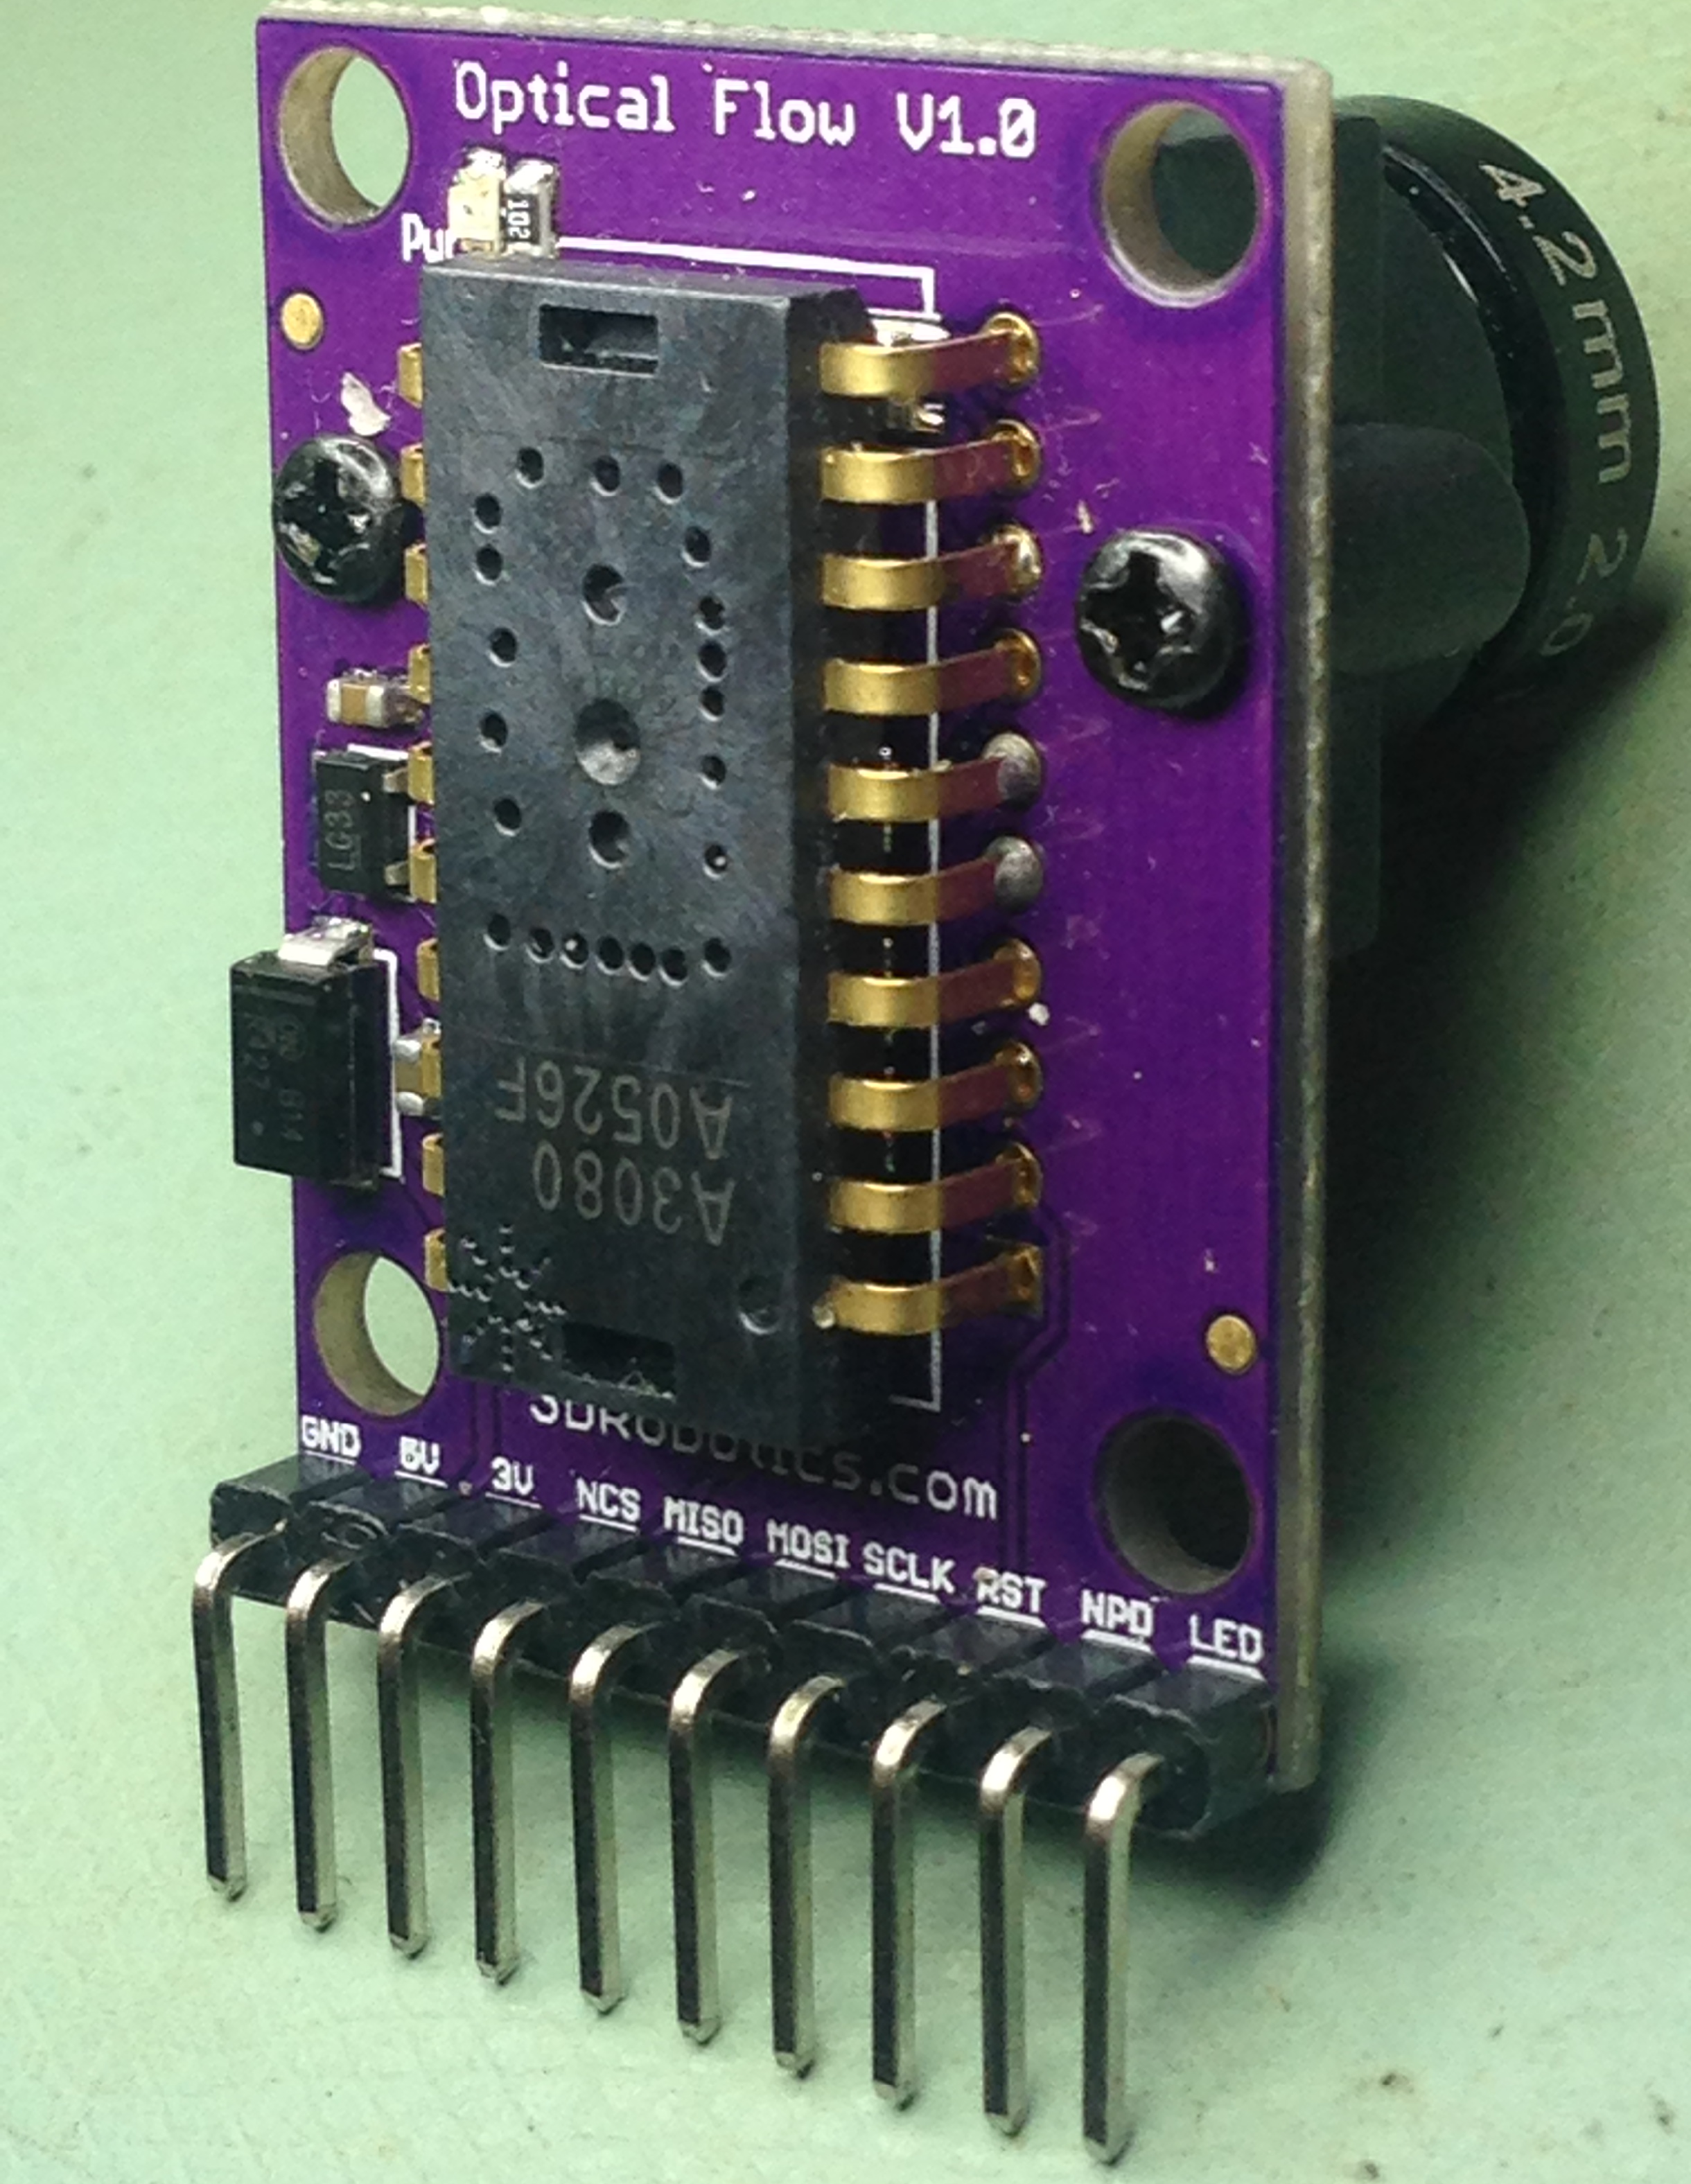
\includegraphics[width=0.4\textwidth]{OpticalFlowSensor}
\caption{Optical Mouse Sensor}
\label{OpticalFlowSensor}
\end{figure}%
%
%\subsubsection{Accumulated \(Z^W\)-axis data calibration}
%
Sensor ANDS-3080 has a programmable frame rate of over 6400 fps. With a lens mounted, this optical flow sensor can theoretically adjust its working distance from zero to one meter. Both of the raw 30-by-30 image frame and the calculated motion results could be retrieved from the optical flow sensor in two different working modes. In the \enquote{image burst} mode, the raw 30-by-30 image frames form a 10 fps live video, helping adjust the lens for a better focus. Whereas in the \enquote{motion burst} mode, the calculated motion results offers accumulation data for both of the sensor's \(x\)-axis and \(y\)-axis.
\\\\%
Concretely as shown in figure \ref{MountedTrackingModuleObservingRail}, only the \(y\)-axis accumulated data is used as the accumulated \(Z^W\)-axis data in the world coordinate, whereas the \(x\)-axis accumulation is always zero (no motion on the \(x\)-axis. Employing the \enquote{motion burst} mode, on ever update, the world coordinate \(Z^W\) could be written as%
%
\begin{equation}
%
Z^W = Z^W_0 + ratio*y^{acc} = Z^W_0 + ratio*(y_{\text{\_all\_previous}} + y_{\text{\_new\_updated}})
%
\end{equation}
%
where \(Z^W_0\) denotes the beginning point of accumulating (concretely at the closest end of the rail to dots pattern), \(ratio\) maps the \enquote{unit one} from \(y\)-axis to the \(Z^W\)-axis, \(y^{acc}\) denotes the accumulated \(y\)-axis movement by data retrieved from the optical flow sensor, which equals to the sum of all previous values and the new updated value.
%
%\subsection{Bluetooth Low Energy for wireless communication}
%
ZigBee, Bluetooth, and Bluetooth Low Energy (BLE) are three most commonly used Personal Area Network (PAN) wireless standards to choose from when wireless communication is needed. ZigBee runs on a mesh topology network (star and point-to-point are the other two basic topologies), which means that the information travels on a web of multiple nodes. Whereas Bluetooth and BLE are famous as point-to-point networking standard, which suits better for this project, from Optical-Flow sensor to PC.
\\\\%
There are huge differences between BLE and \enquote{classic} Bluetooth; despite falling under the same name, they are entirely different technologies. Bluetooth consumes more power and transmits farther and with more data. It is suited for streaming media such as playing music on Bluetooth speakers or taking a call through a Bluetooth headset.
%
\begin{figure}[H]
\centering
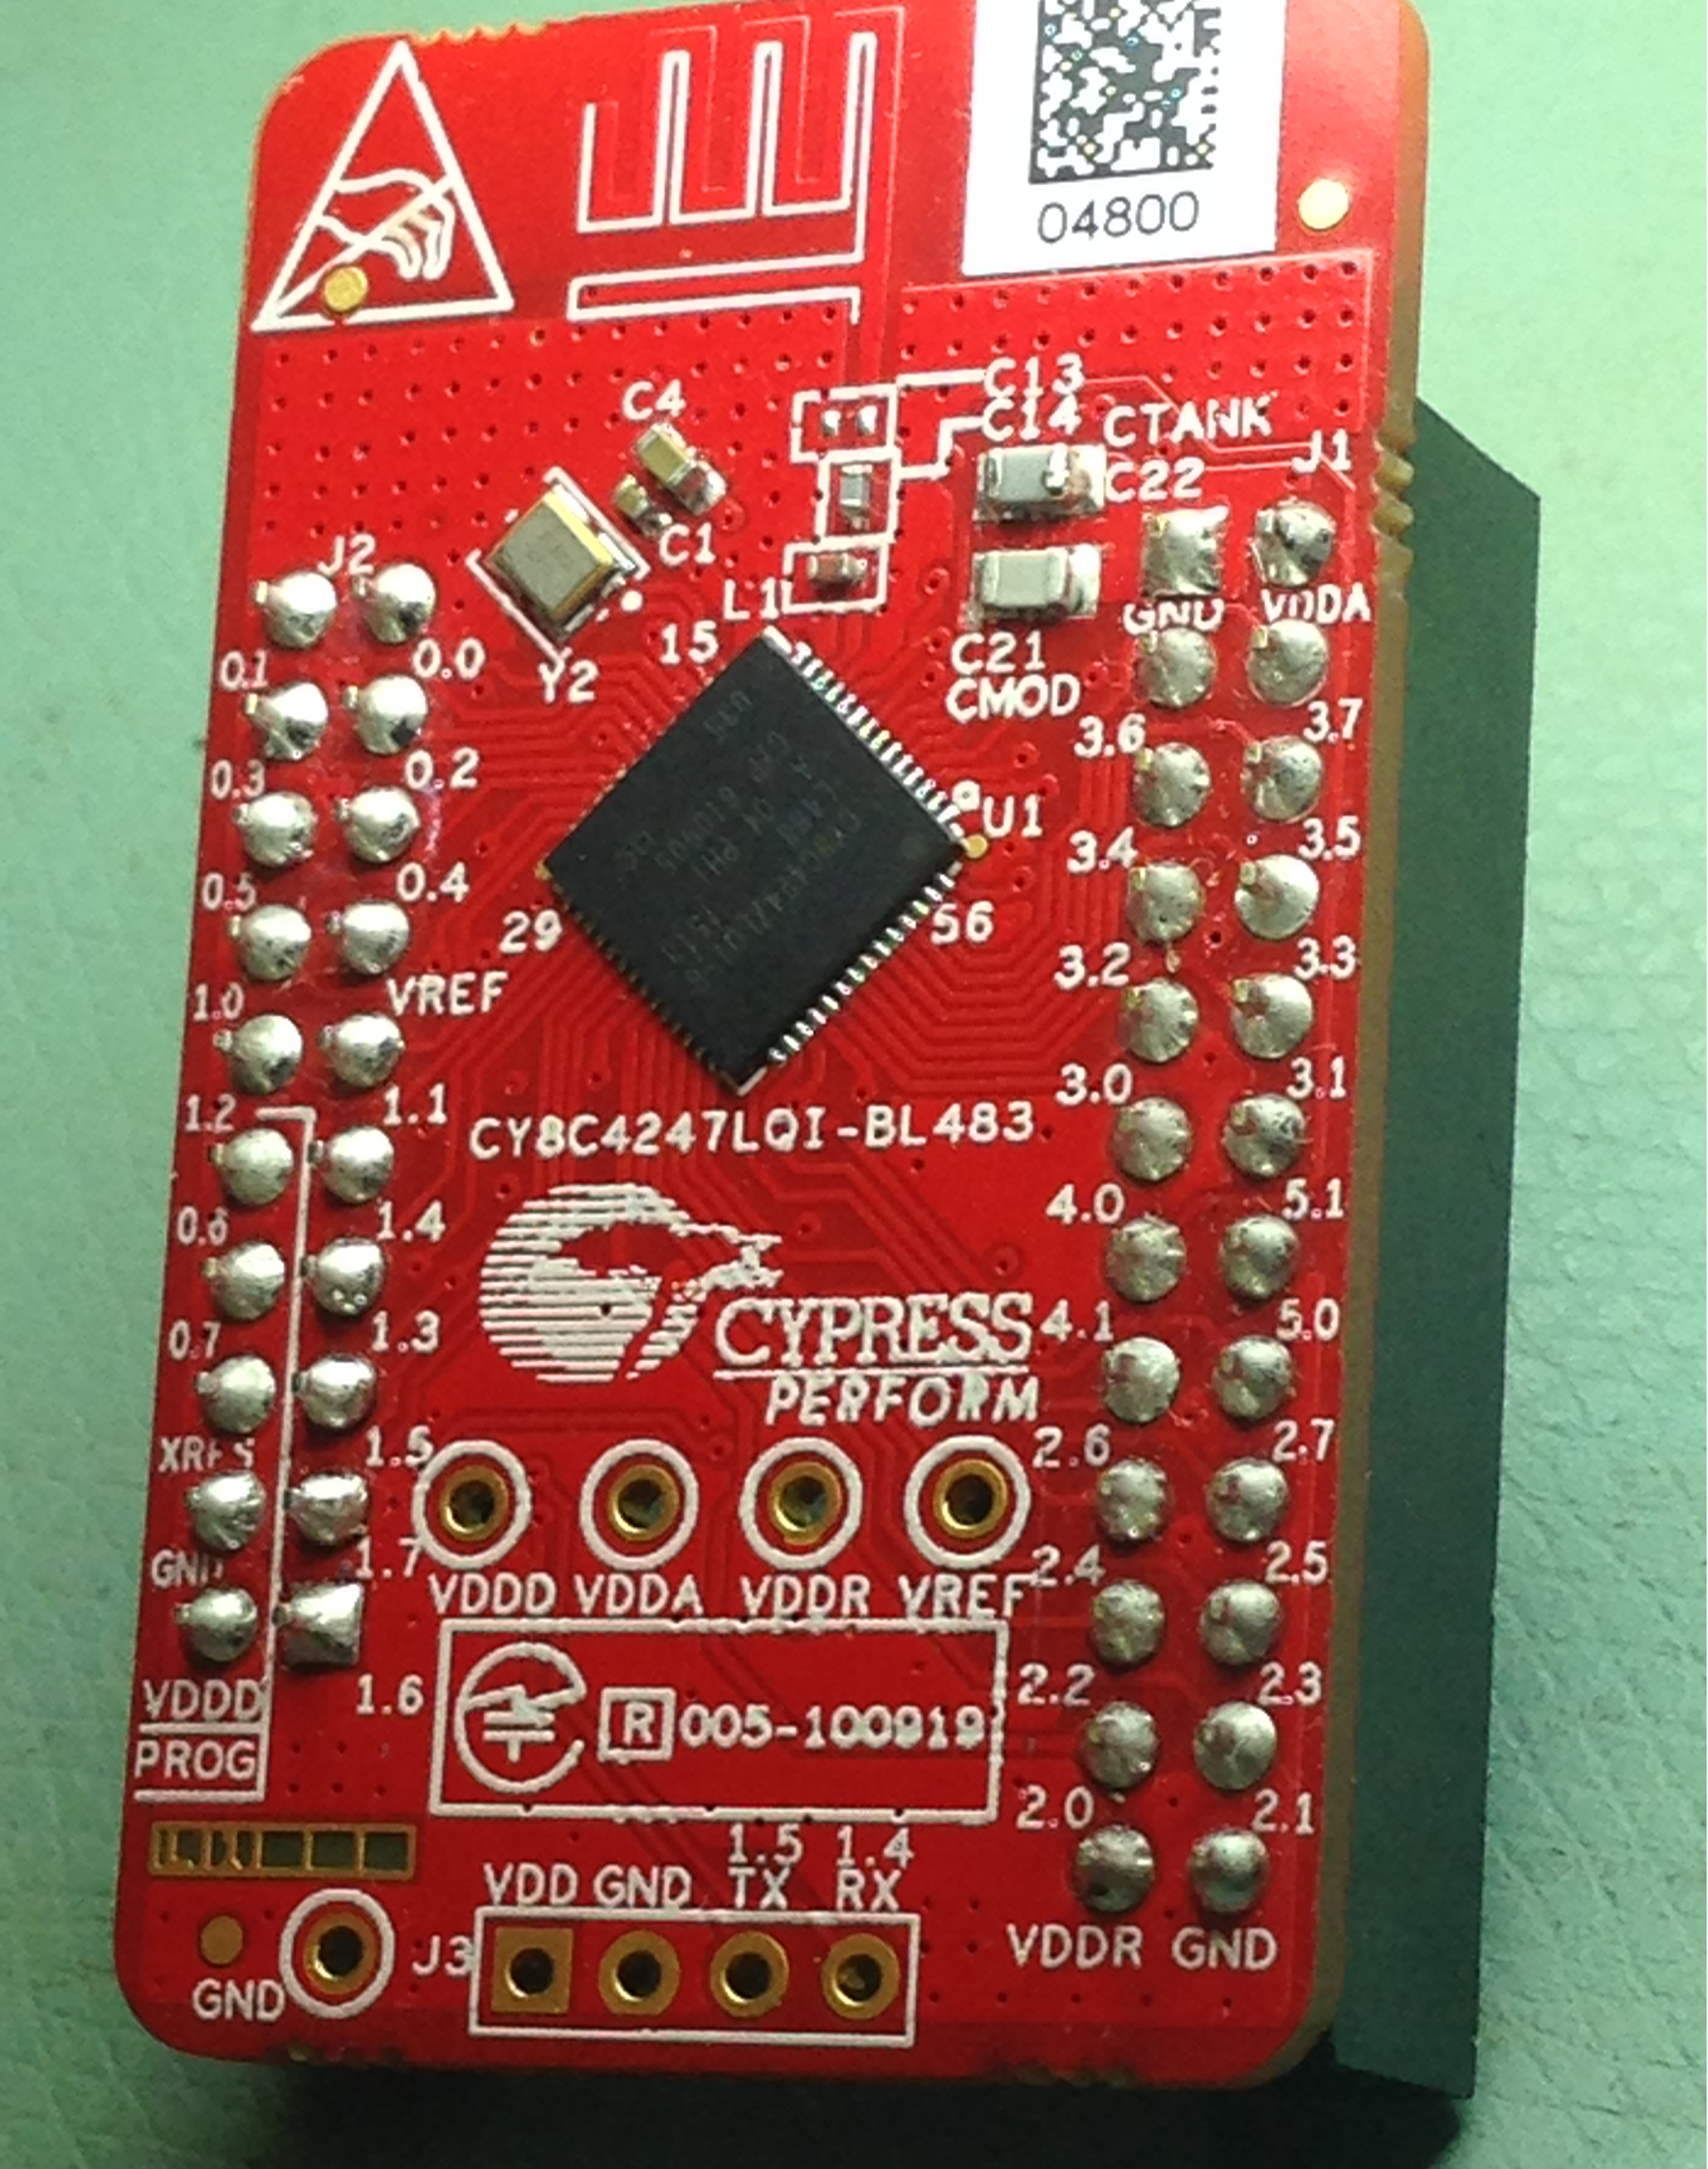
\includegraphics[width=0.4\textwidth]{PSoC_BLE_Module}
\caption{Cypress PSoC BLE Module}
\label{PSoC_BLE_Module}
\end{figure}%
%
Whereas BLE transmits less data over shorter distances using much less power than Bluetooth. Both of the transmission frequency and the amount of data to transfer per time are controllable by developer for BLE communication.
\\\\
%
As for the wireless data transmission in this project, with the \(x\)/\(y\) accumulation data being to transfer, the amount of data to transfer per time is only two bytes. Moreover, the maximum frame rate of optical flow sensor ANDS-3080 is 6400 fps, which means the transmission frequency cannot be faster than 6400 Hz (we do not need that fast in the meantime). In short, BLE is finally chosen as the wireless networking to transfer data from the optical flow sensor to PC. Concretely, the Cypress PSoC BLE Module is used, with a 10KB maximum throughput that is enough for the demand in this project, as shown in figure \ref{PSoC_BLE_Module}.
%
%\subsubsection{BLE Programming based on Protocol}
%
BLE is a low-power, short-range, low-data-rate wireless communication protocol. Unlike Bluetooth application that only the high level connection needs to be concerned, the BLE application developing needs low level programming, more complex but offering more control space for developer. Figure \ref{BLE_Protocol_Stack} shows the BLE Protocol Stack that BLE developers need to refer to.
%
\begin{figure}[H]
\centering
\includegraphics[width=0.7\textwidth]{BLE_Protocol_Stack}
\caption{BLE Protocol Stack \cite{Cypress15}}
\label{BLE_Protocol_Stack}
\end{figure}%
%
Cypress BLE Module helps handle the lowest hardware controller section (PHY, LL, HCI) and part of the firmware host section (L2CAP, ATT, SM), so that developers only need to take care of the GAP and GATT layers. GAP provides an application-oriented interface that determines whether the device acts as a BLE link \enquote{Central} or \enquote{Peripheral}, and configures the underlying layers accordingly. Whereas GATT defines methods to access data defined by ATT layer ( \enquote{Client} to receive or \enquote{Sever} to send).
\\\\%
Concretely for the BLE programming in this project, on the GPA layer, the BLE module continuously retrieving data from Optical-Flow sensor is the \enquote{Peripheral} that advertises to a Central, while a BLE dongle (receiver connected on PC) is the \enquote{Central} that scans for advertisements from GAP Peripherals and is going to establish the connection with the BLE module. Whereas on the GATT layer, the BLE module is the \enquote{Sever} that contains data and the dongle on PC works as a \enquote{Client} to receive data.
\\\\%
To program on the PC side, both of the command sending and data receiving are through the serial port which connects the BLE dongle. Both of the output command to send and received the input data are packaged in a center format, which means for every command about BLE control, there must be a method to package it and a corresponding decoding method to extract valid data. All of the commands that need to be managed are to handle GATT data transmission and GAP connection problem. After GATT and GAP setting, concretely, the optical flow sensor works at a sampling rate of 2000Hz and the BLE communication speed is 100 updates per second, i.e., \(Z^W\) is updated at 100Hz.
%
%
\subsection{PCB Joint, Power Supply and Illumination}
%
Figure \ref{SenSinglePCB} shows the PCB combining and powering (3.3 \texttildelow \, 16V flexible voltage input) for a PSoC BLE module, an OF sensor, and a LED for OF sensor illumination. Figure \ref{BLE_OF_TrackingModule_Overview} shows the overview of the BLE Optical-Flow Tracking Module.
%
\begin{figure}[H]
\centering
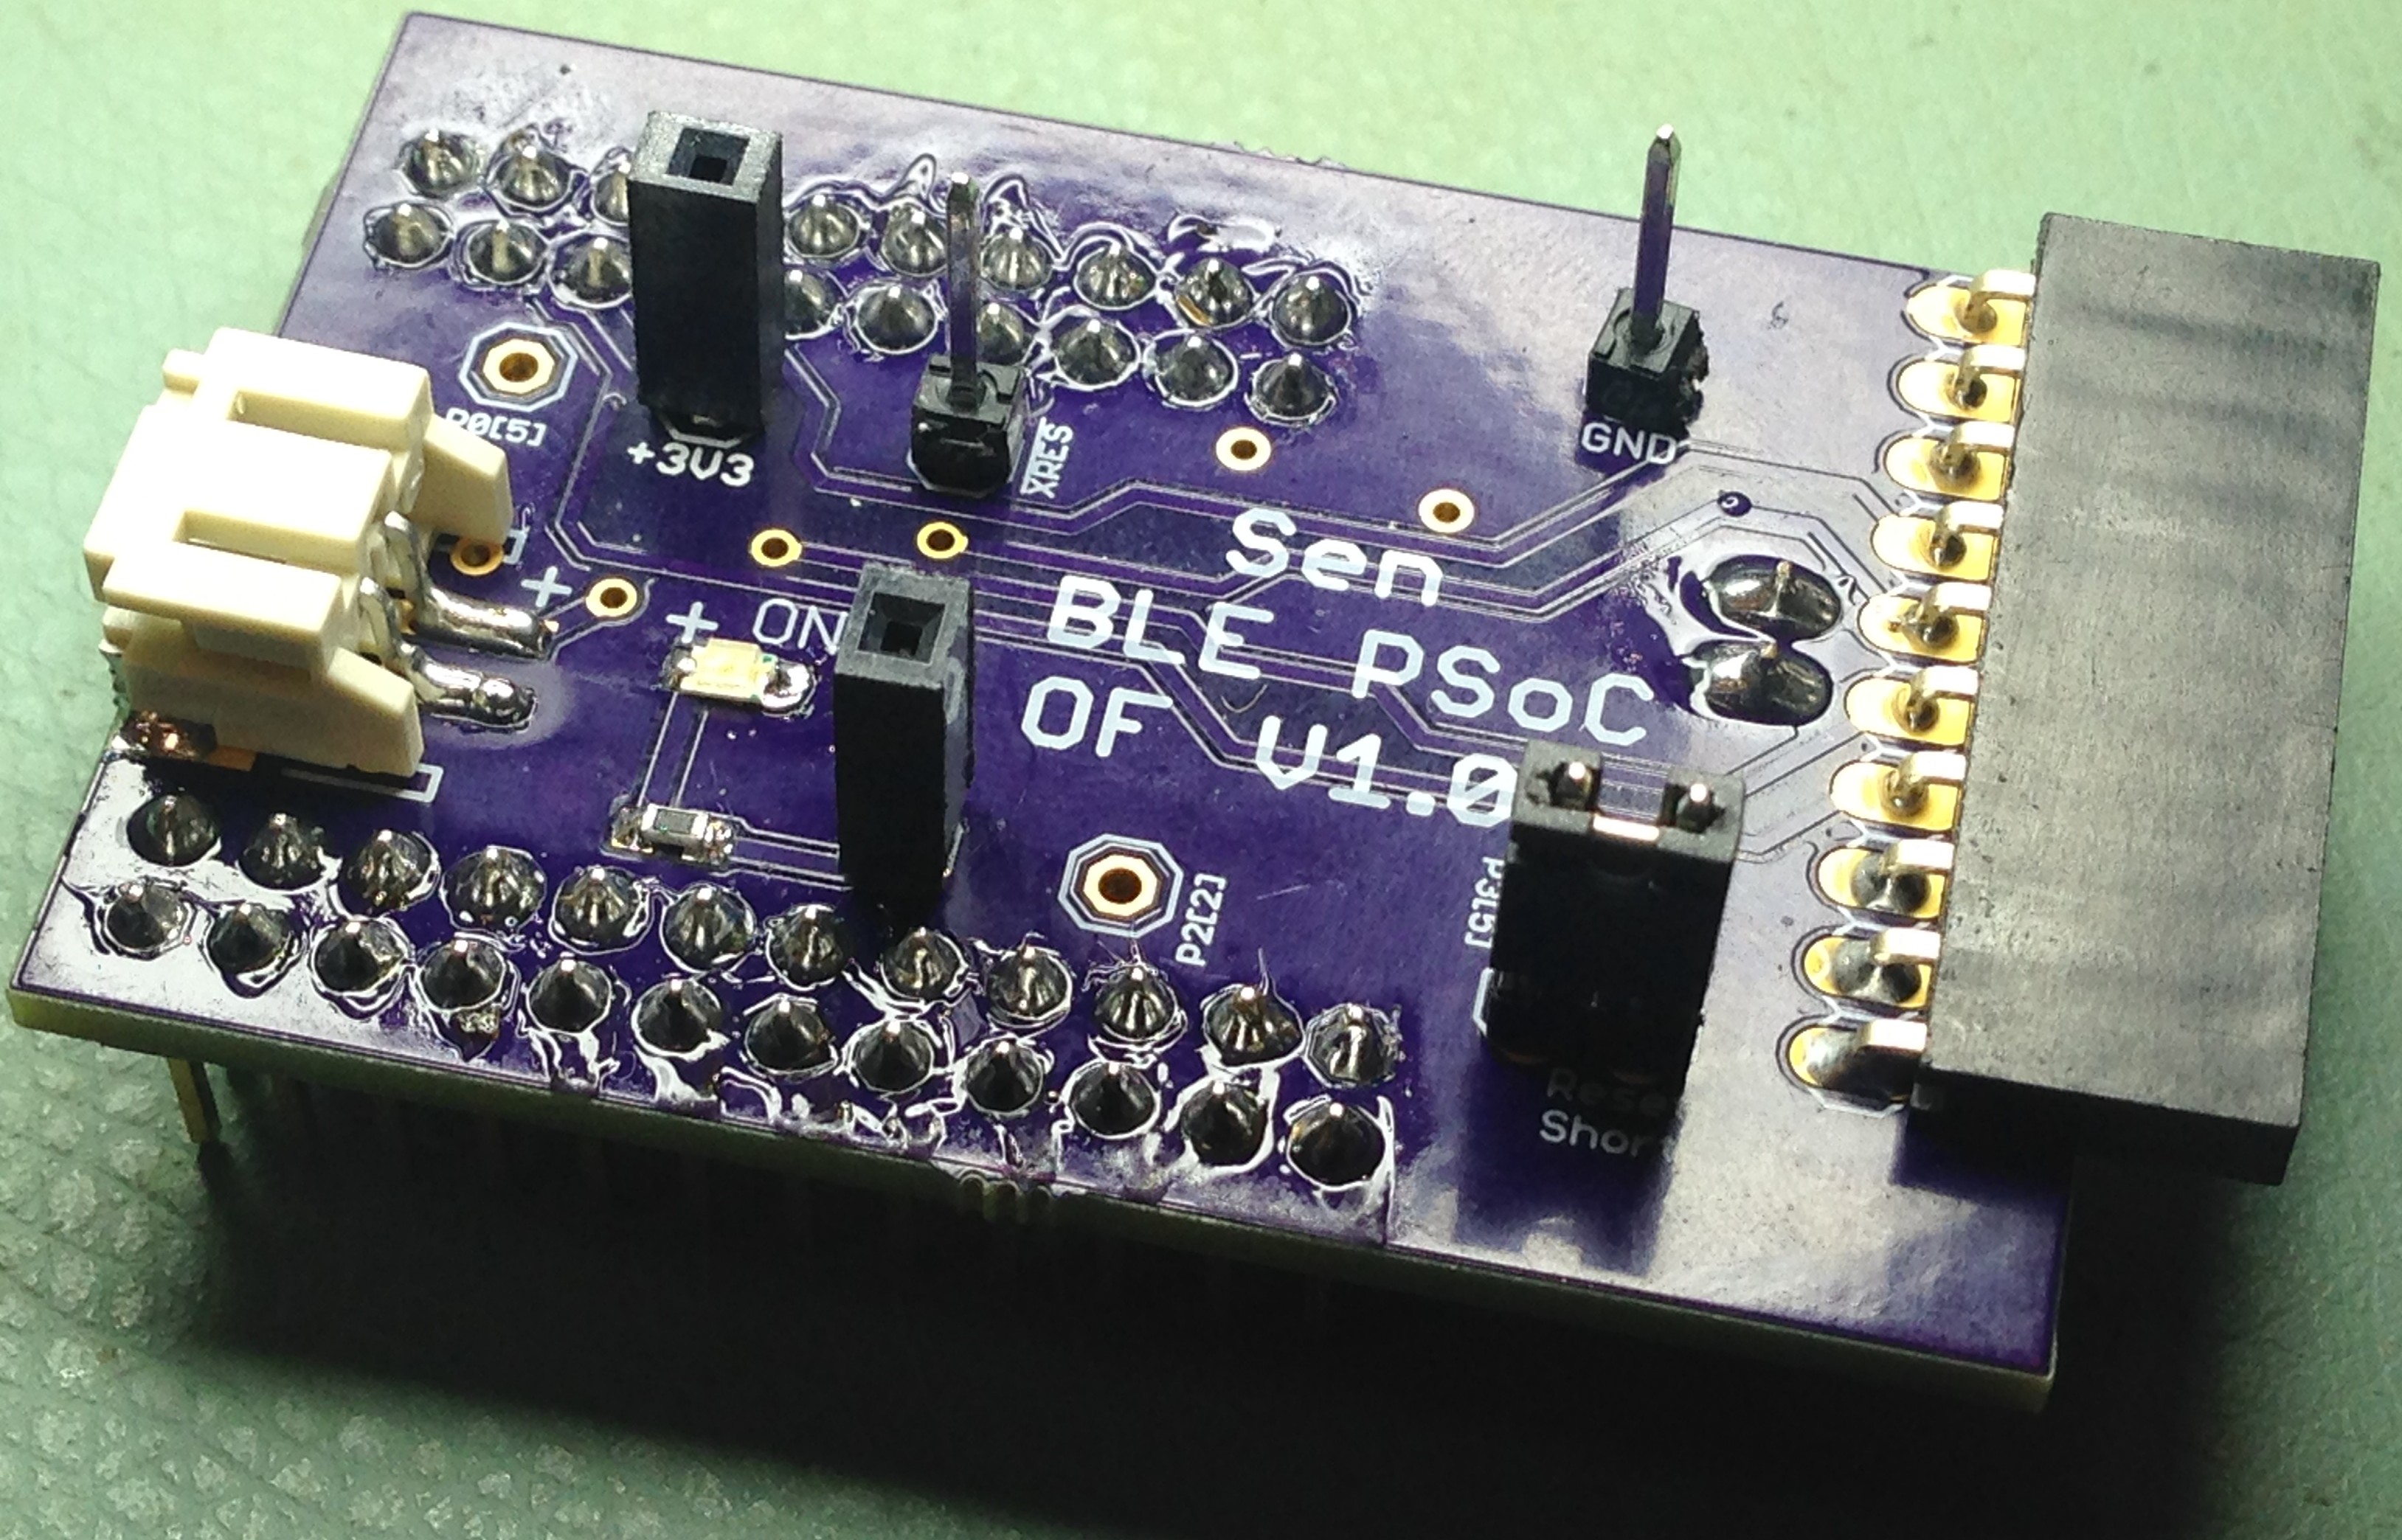
\includegraphics[width=0.7\textwidth]{SenSinglePCB}
\caption{PCB: joint \& power supply}
\label{SenSinglePCB}
\end{figure}%
%
%
 \begin{figure}[H]
\hspace*{-0.3cm}
\centering
\subfloat[Front Side][Front]{
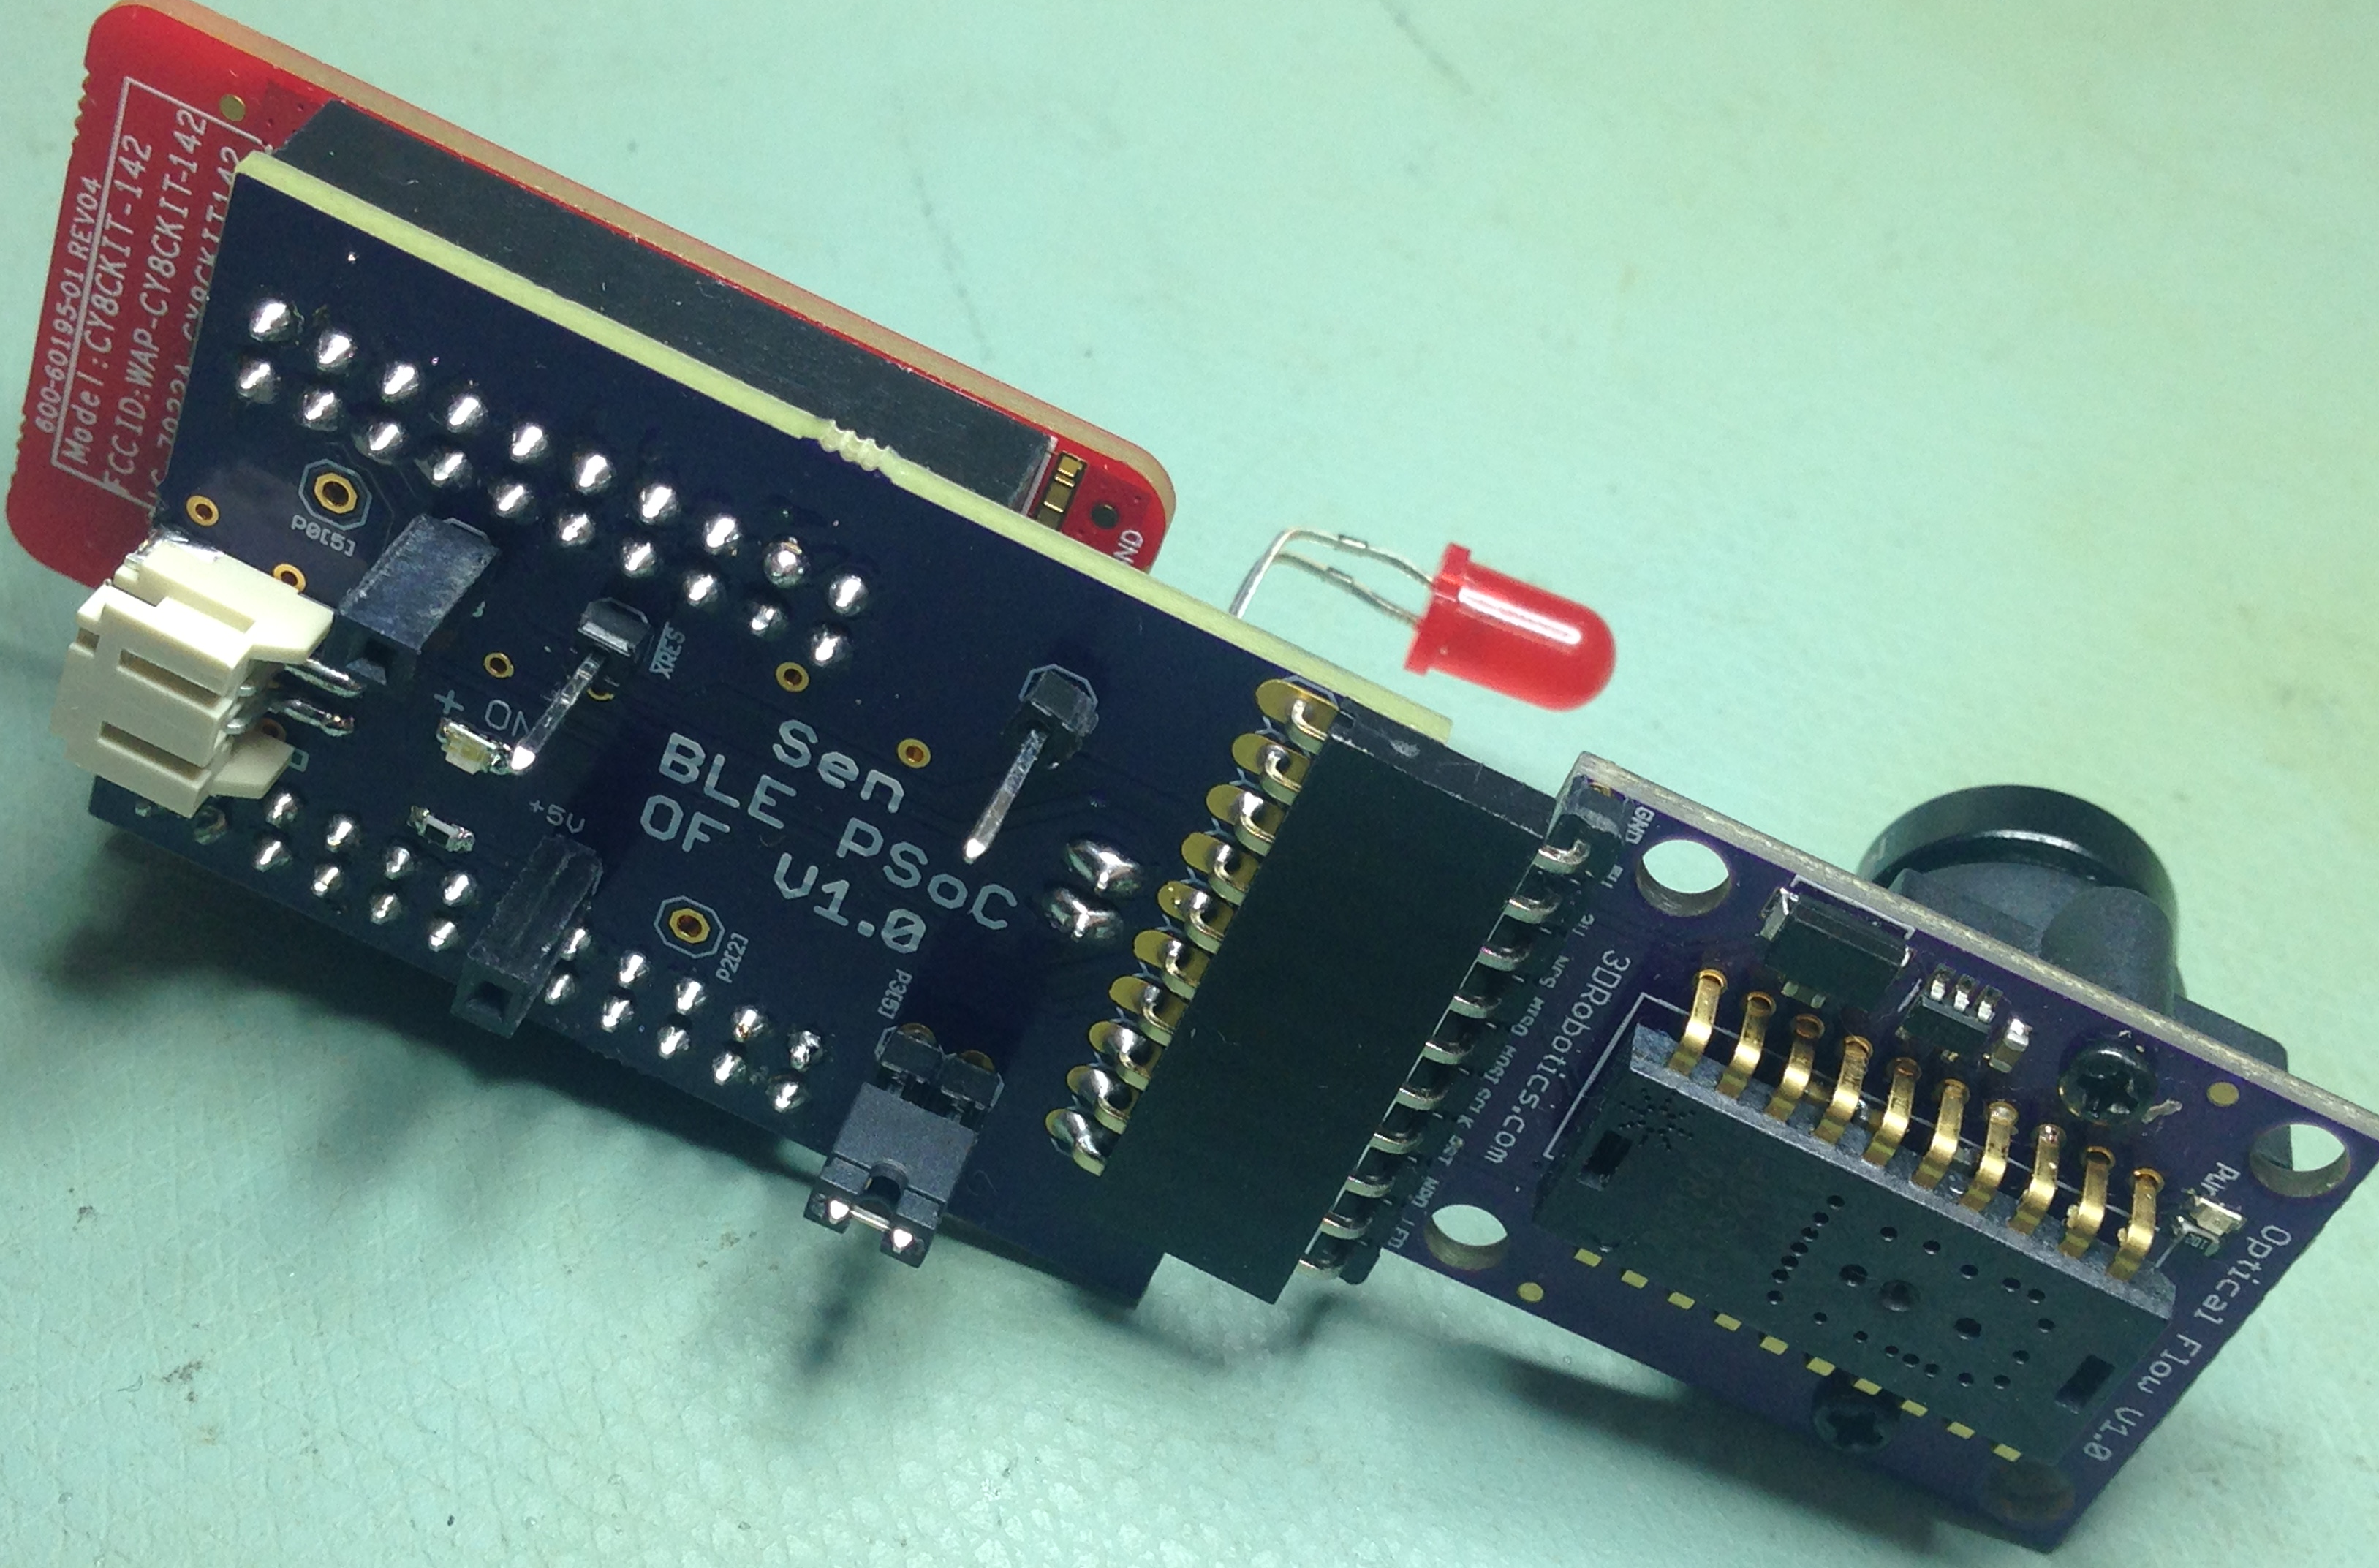
\includegraphics[width=0.54\textwidth, height = 0.35\textwidth]{combinedModuleFace}
\label{combinedModuleFace}}
%\qquad
\subfloat[Back Side][Back]{
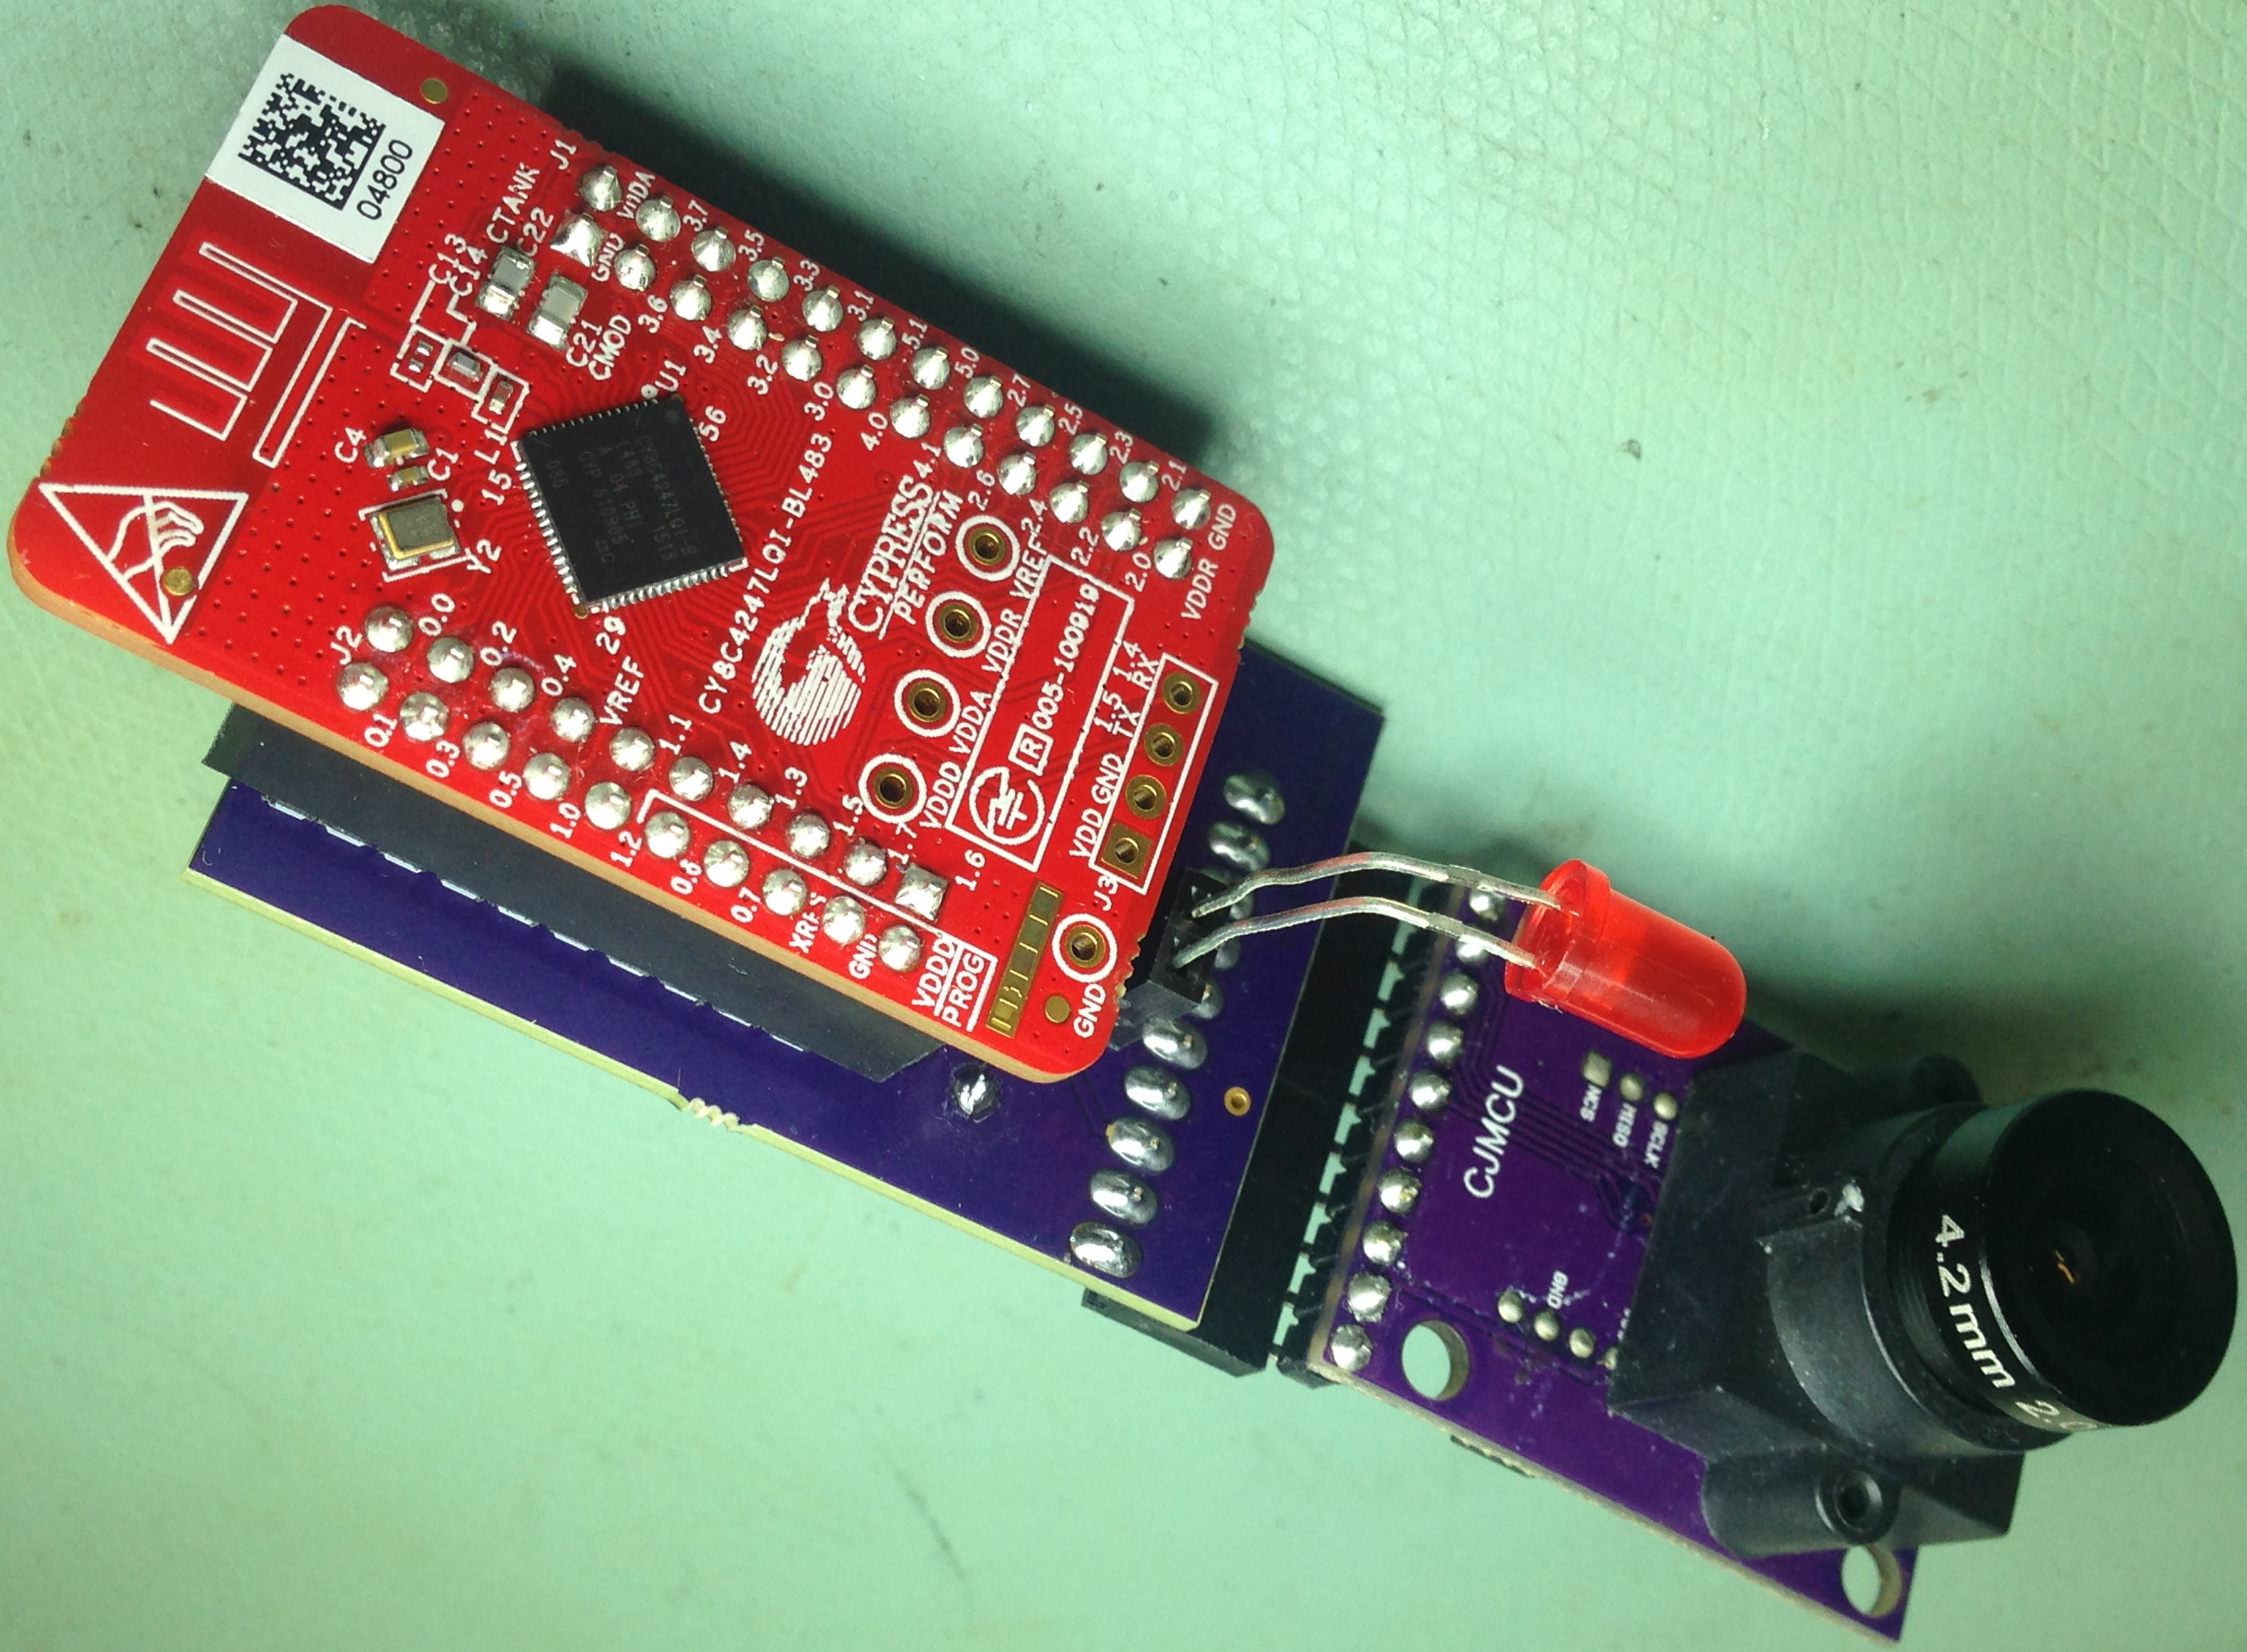
\includegraphics[width = 0.47\textwidth, height = 0.35\textwidth]{combinedModuleBack}
\label{combinedModuleBack}}
%
\caption{Overview of BLE OF Tracking Module}
\label{BLE_OF_TrackingModule_Overview}
\end{figure}%
%
%
%
%
%
%
%
%Chapter 4: results for 3 types of RGB-D cameras.\\
%Chapter 5: conclusion\\





































